\section{Results}
\label{sec:Auswertung}

\subsection{Laser Mode}

As the first step we determine the current treshold from which on the diode is in laser mode. To get a visual indication of the transition from LED to laser diode a IR viewing card is placed in front of the laser. This card emitts light in the optical spectrum if infrared light hits it. We observe this light with the video of the camera on a screen. For the wide spectrum of the LED mode it shows a rather clean circle. When the diode enters laser mode a speckle pattern is seen. Then we lower the current slightly under this laser treshold and optimize the positioning of the gatter in terms of the vertical orientation. This increases the amplification by the aforementioned external cavity. When the speckle pattern is seen again we lower again the current a bit. After a few iterations of these two steps the laser is in an optimal condition for the next step. The voltage of the treshold is $U_\text{t} = \SI{3.42(1)}{\volt}$ and because of the inner resistance of $R_\text{i} = \SI{100(1)}{\ohm}$ the current is $I_\text{t} = \SI{34.2(4)}{\milli\ampere}$.

\subsection{Florescence}

In the next step we try to reach the wavelength which fits the energygap in the absortion spectrum of the rubidium gas. To change the wavelength of the laser we change the current which is applied to it. This changes the temperature of the semiconductor and therefore its bandgap. In addition the reflectionindex changes. These effects result in a different overall wavelength and a different "free spectral range" because of formel \eqref{eqn:???}.

The pictures in figure \ref{fig:fluo_no_fluo} show the difference it makes when the laser hits the right wavelength. Then a clear beam of florescence is seen. The right one was achieved with a voltage of $U_\text{f} = \SI{5.33(1)}{\volt}$ and this means a current of $I_\text{f} = \SI{53.3(5)}{\milli\ampere}$ with the same resistance as above.

\begin{figure}
  \centering
  \begin{subfigure}{0.45\textwidth}
    \centering
    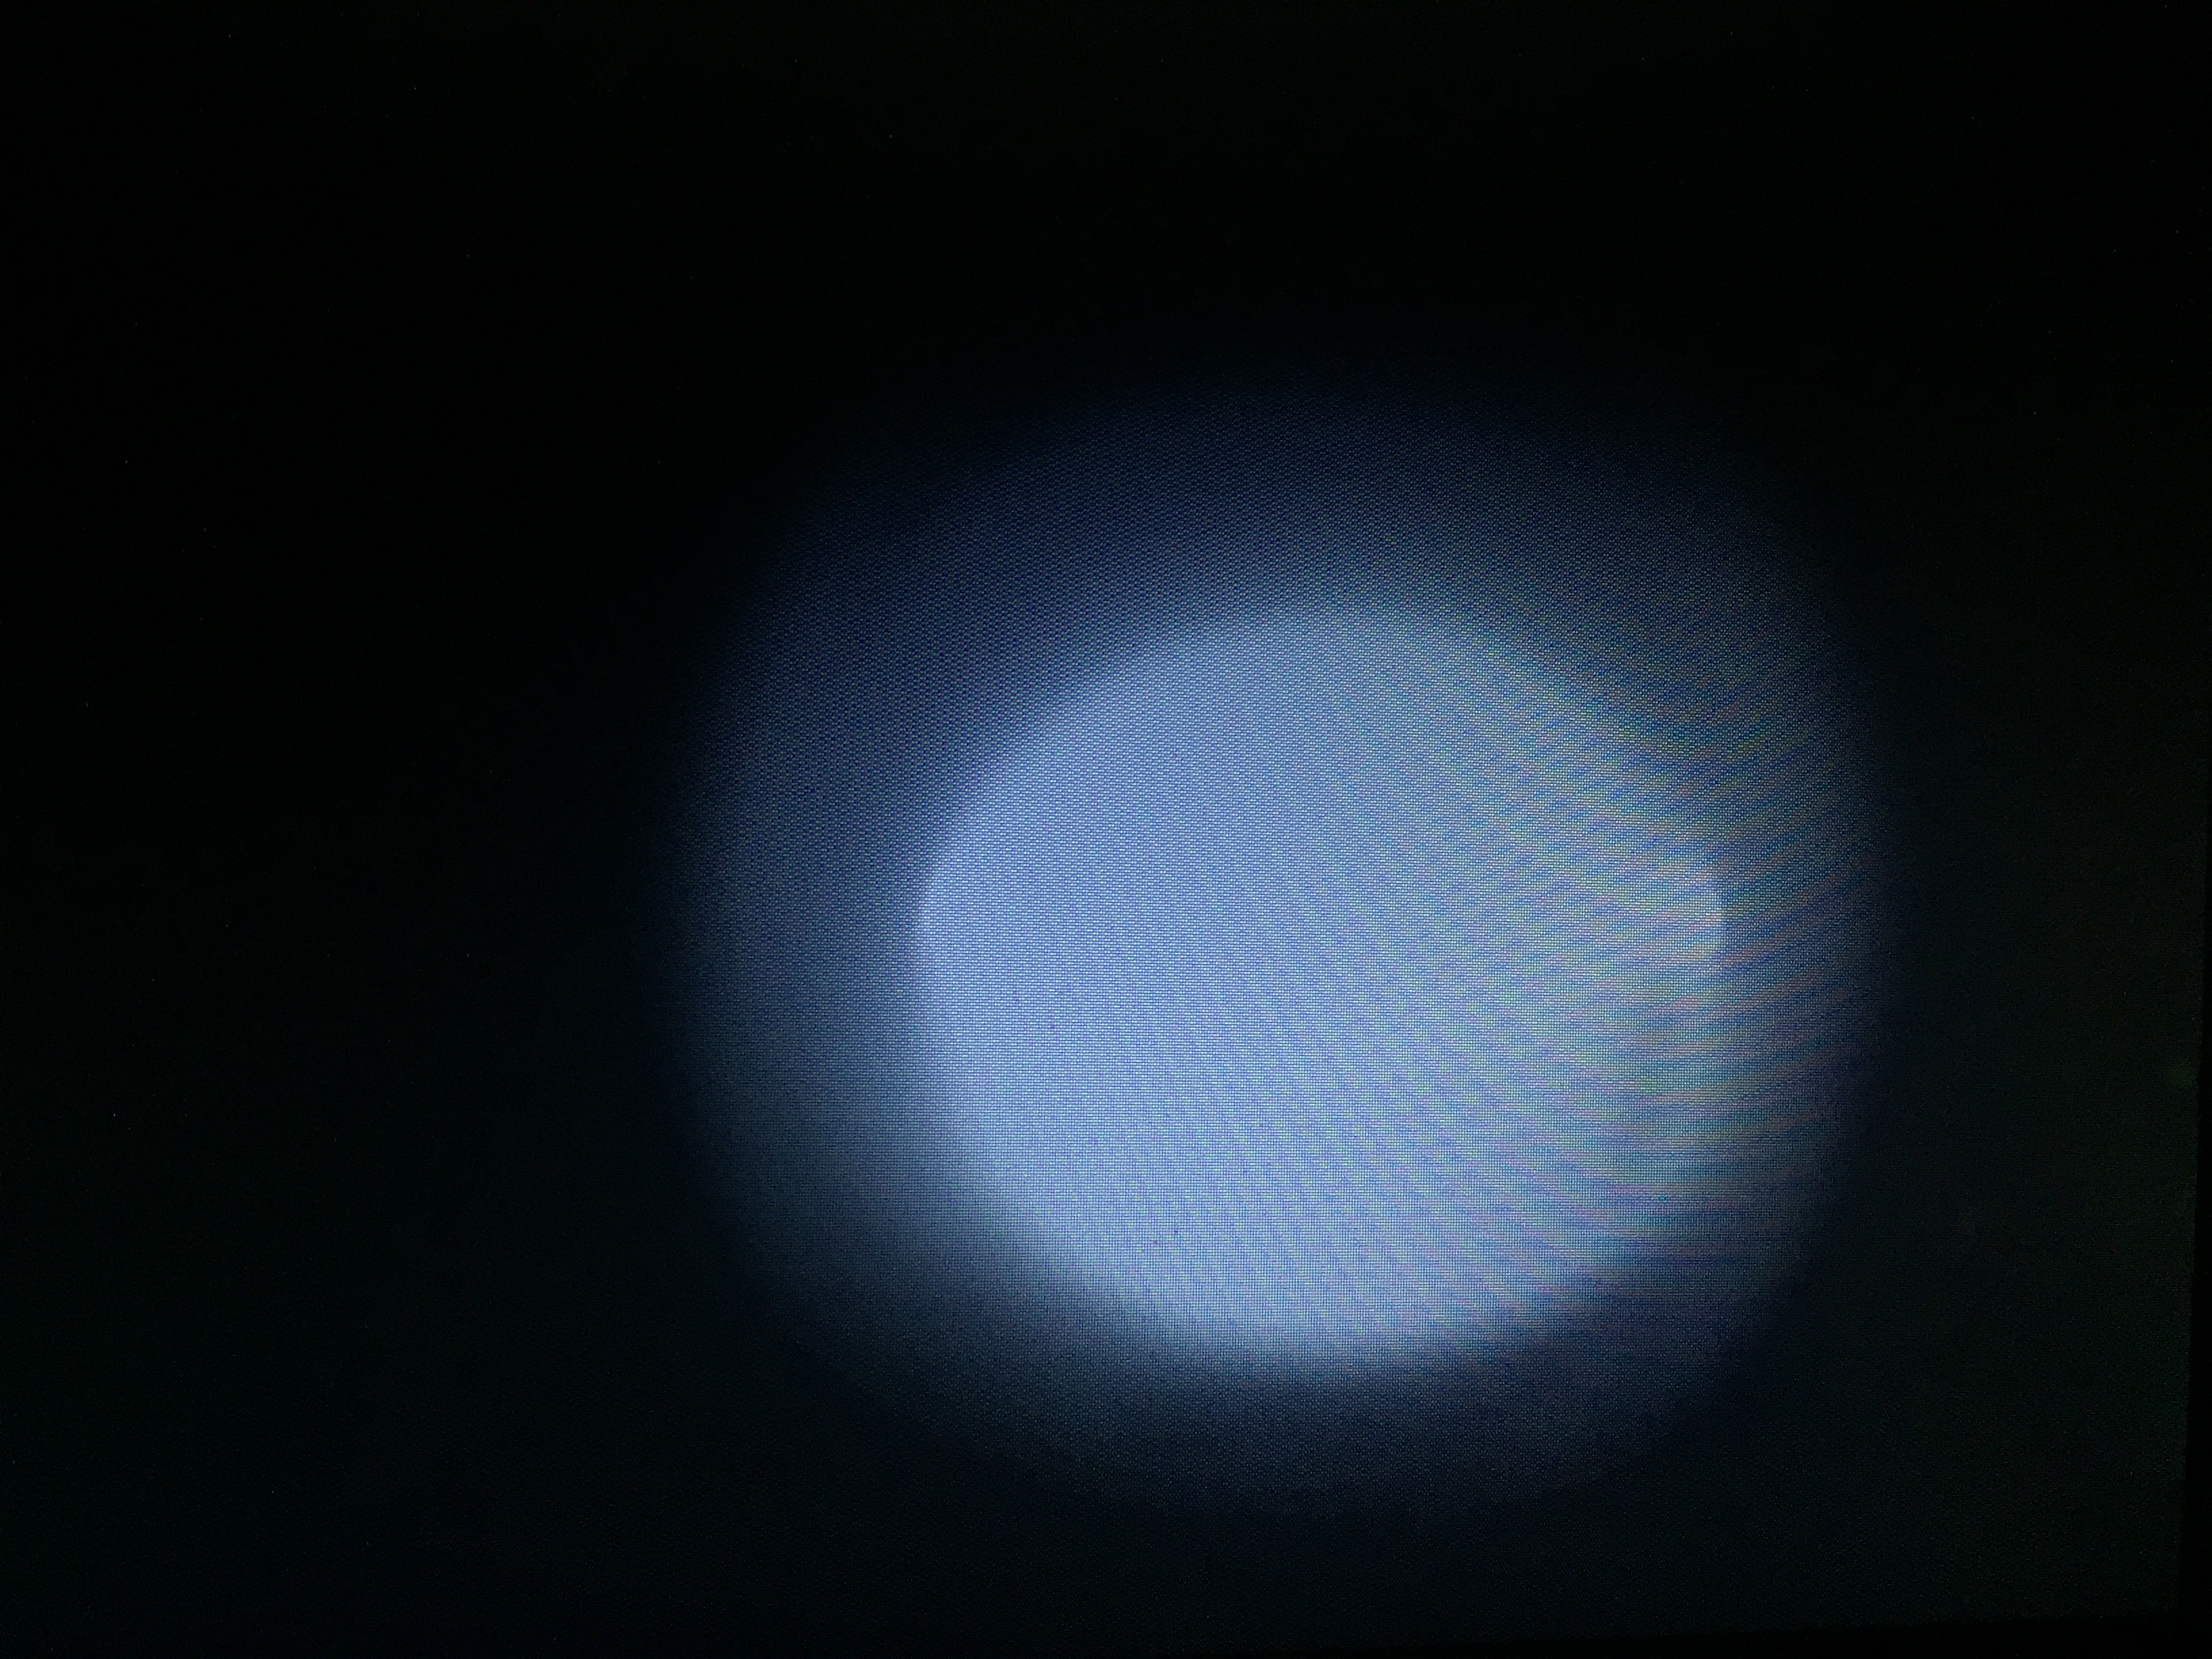
\includegraphics[height = 4cm]{pics/no_fluo.jpg}
    \caption{Cell hit by a wavelength outside of the absorption spectrum.}
    \label{fig:no_fluo}
  \end{subfigure}
  \begin{subfigure}{0.45\textwidth}
    \centering
    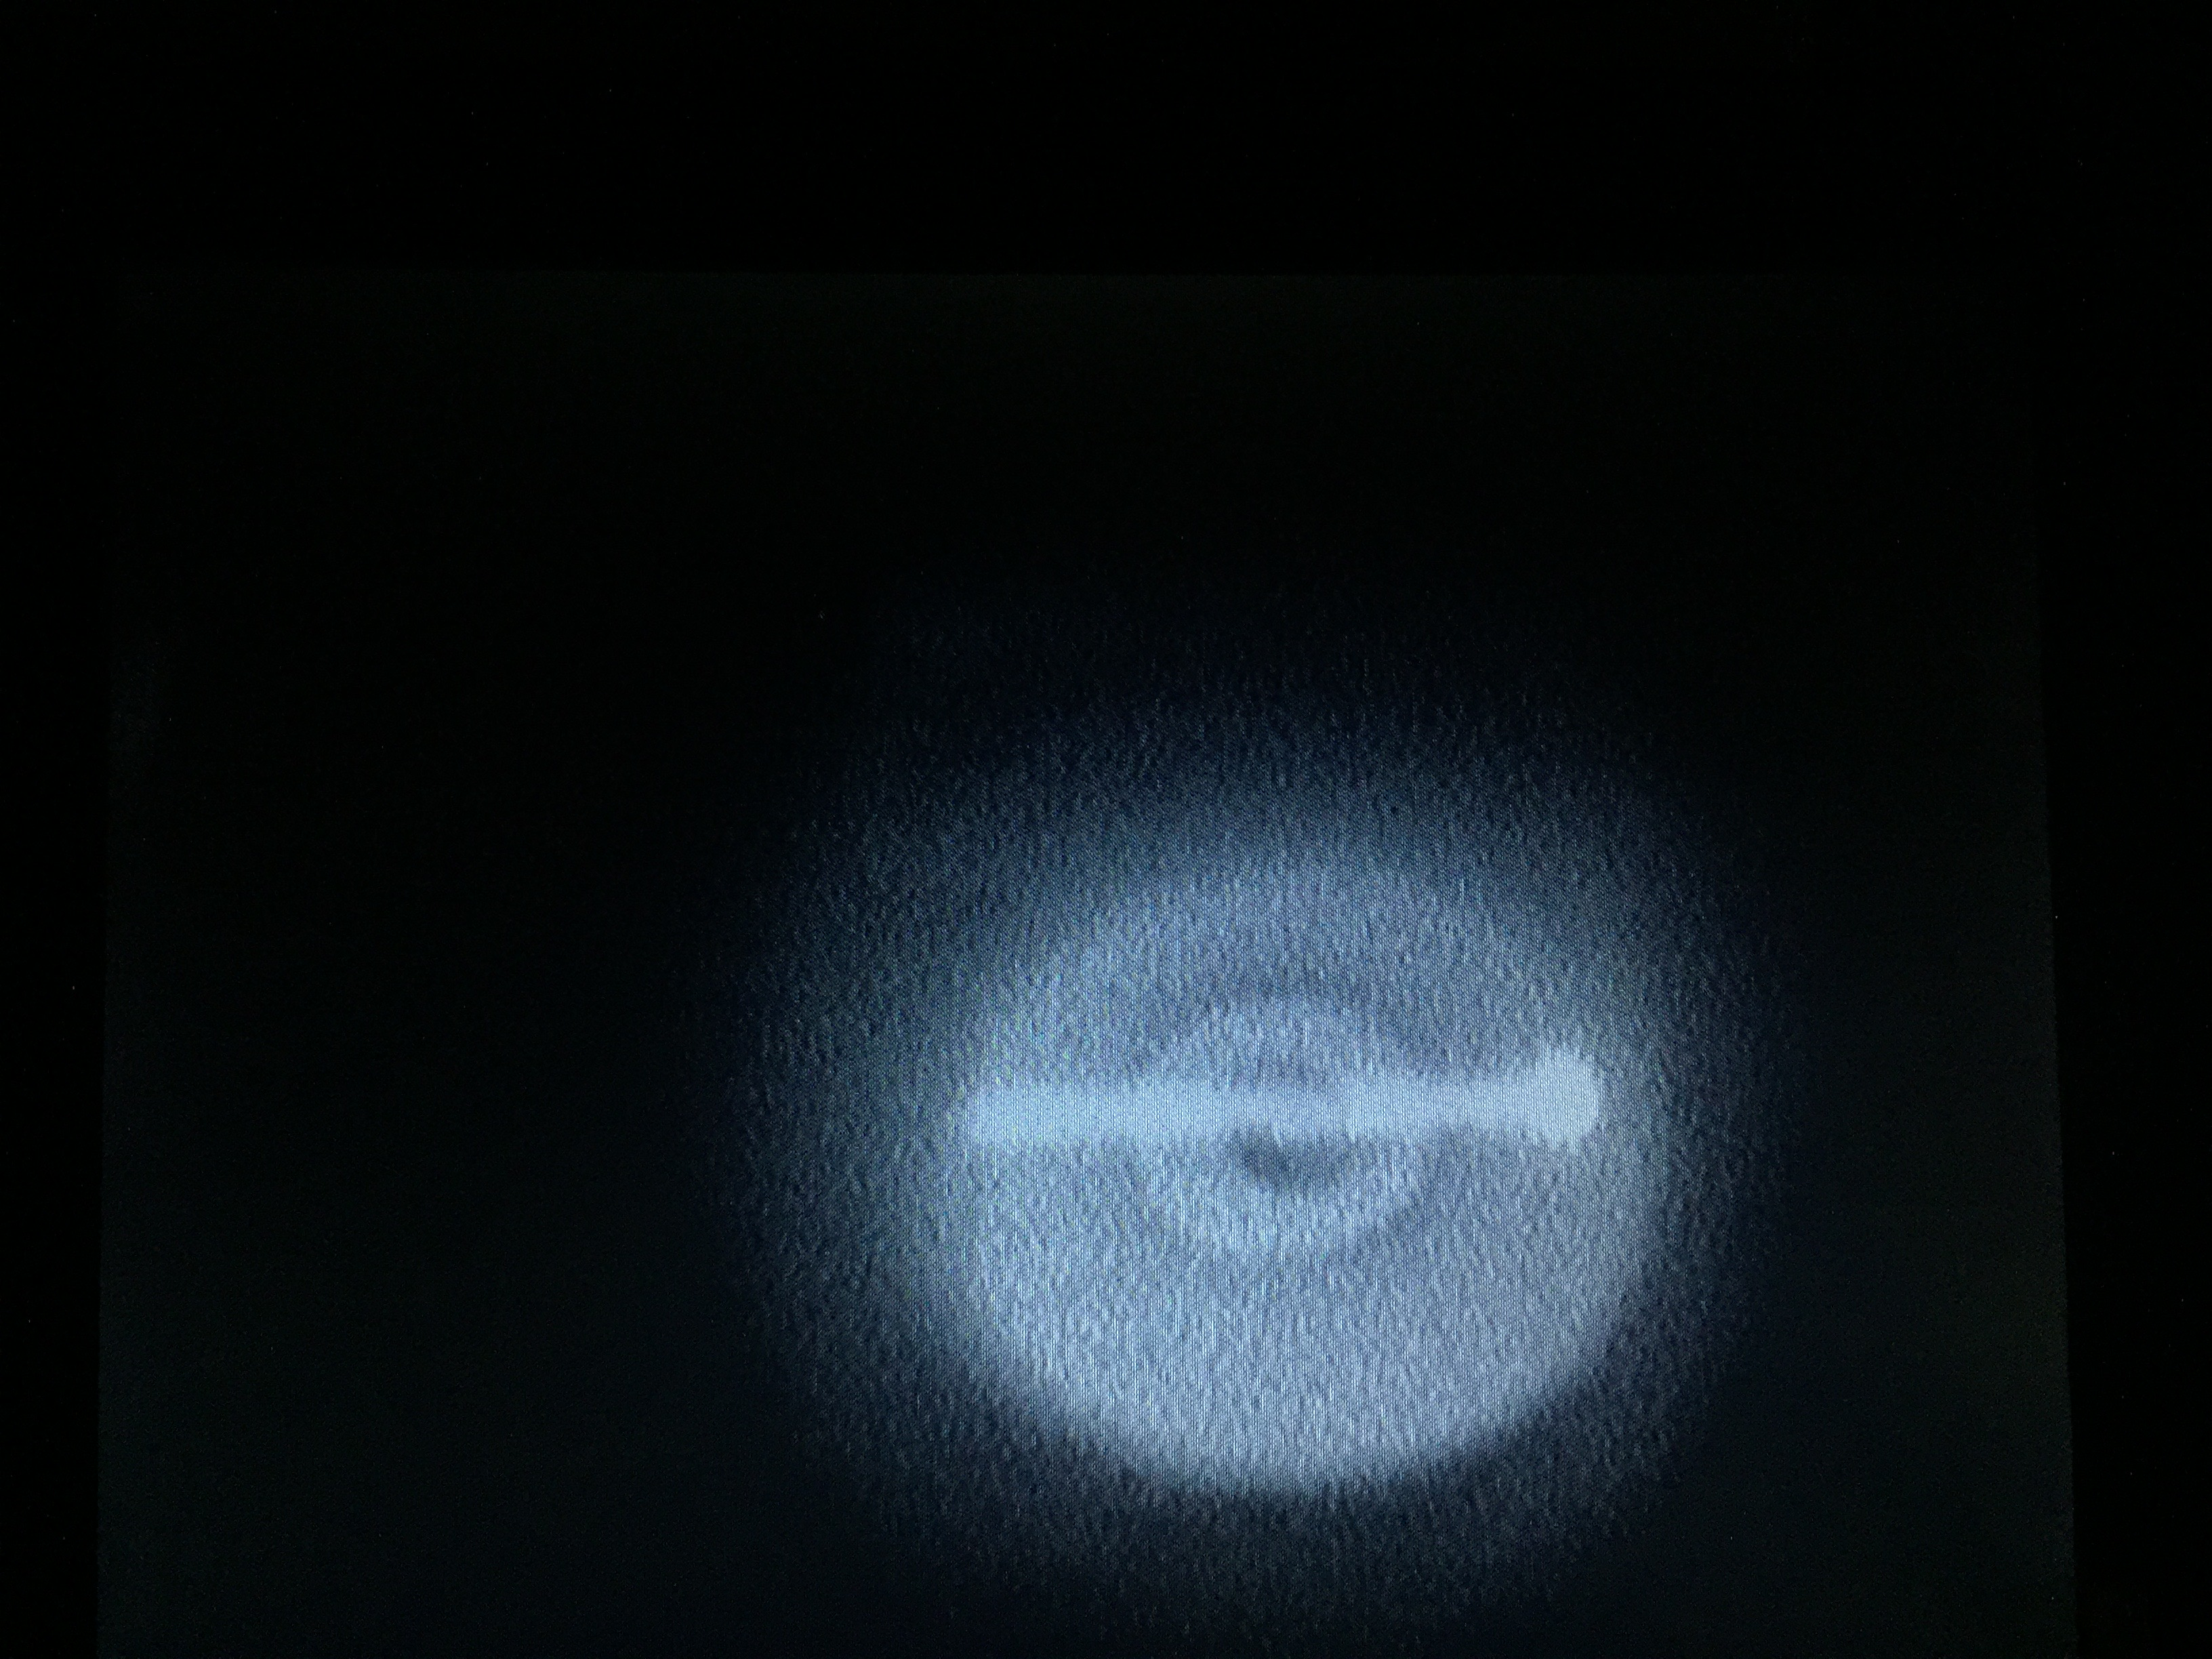
\includegraphics[height = 4cm]{pics/fluo.jpg}
    \caption{Cell hit by a wavelength inside of the absorption spectrum.}
    \label{fig:fluo}
  \end{subfigure}
  \caption{Pictures of the rubidiumcell enlightened by different wavelengths.}
  \label{fig:fluo_no_fluo}
\end{figure}

\subsection{The Absorption Spectrum of Rubidium}

Now that we obtained a laser with a fitting intensity and a wavelength near to the absorption spectrum the next step is to loop over a few different wavelengths to record the whole spectrum. To achieve this we connect a ramp generator to the piezo controller. This enlargens the piezoelectric stack which moves the gatter therefore vary the length of the external cavity and results in a periodically changing wavelength. In figure \ref{fig:triangle_with_absorption} the voltage applied to the piezo monitor and the signal of one photodiode after the cell is shown. The signal of the photodiode may be a bit wrong because at this part of the experiment the laser did not hit the diode completely.

\begin{figure}
  \centering
  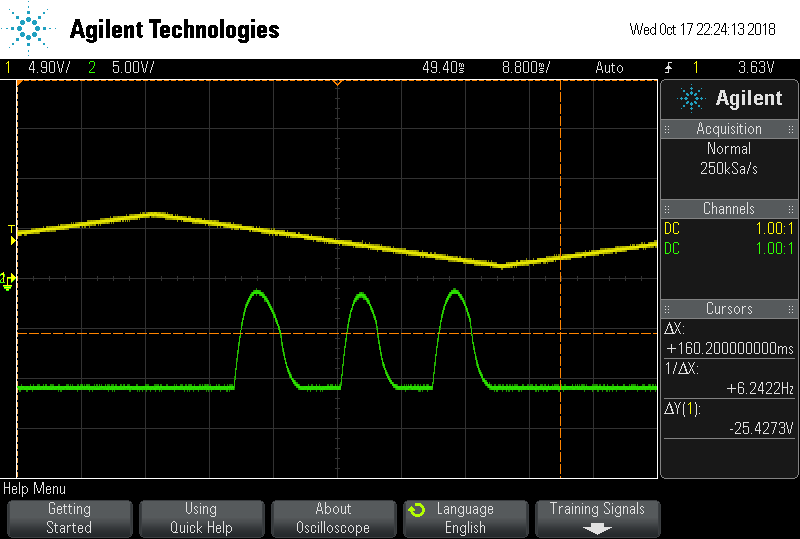
\includegraphics[height = 5cm]{pics/scope_199.png}
  \caption{Voltage on the piezoelectric stack and some absortion dips from one photodiode.}
  \label{fig:triangle_with_absorption}
\end{figure}

Now we connect the ramp generator besides its connection to the piezo controller also to the laser current. This allows a larger scan area without mode hops. With the right settings figure \ref{fig:dreieck_mit_absorption} is shown on the oscilloscope screen.
\begin{figure}
  \centering
  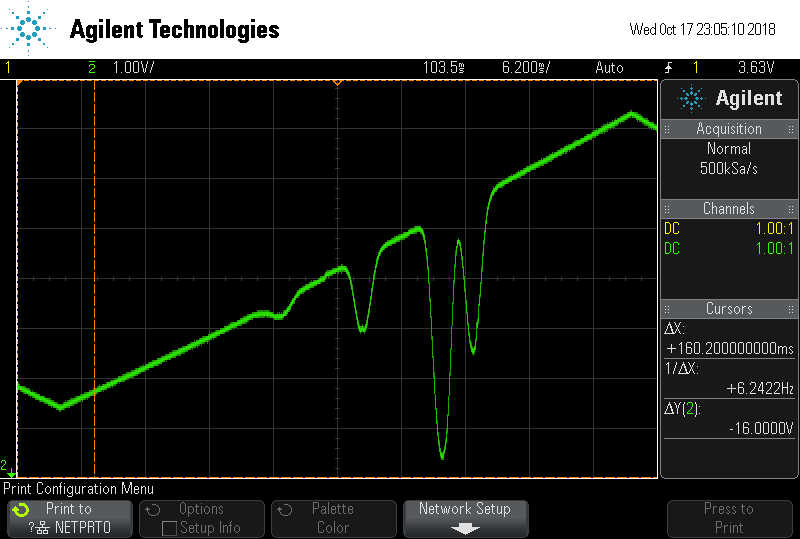
\includegraphics[height = 5cm]{pics/dreieck_mit_absorption.png}
  \caption{Signal of one photodiode with synchronized current and piezo controller.}
  \label{fig:dreieck_mit_absorption}
\end{figure}
To surpress the effect of the changing laser intensity we place a beam splitter in front of the cell which reflects one half of the laser beam to another photodiode. After this we can substract the signal of the laser which went through rubidium, from the laser signal which went directly into the second photodiode. By balancing the two signals with the controls on the subtraction controller a nice picture of the absorption spectrum can be achieved and is shown in figure \ref{fig:perfect_absorption}.
\begin{figure}
  \centering
  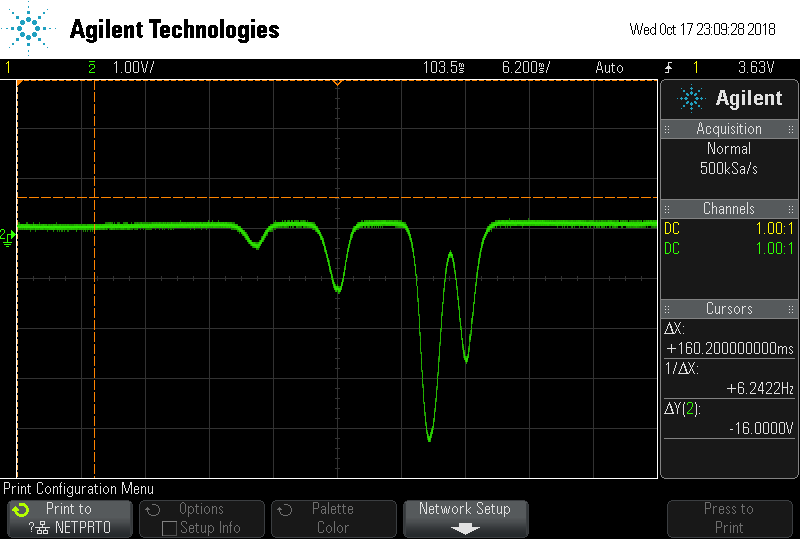
\includegraphics[height = 5cm]{pics/perfect_absorption.png}
  \caption{The recorded absorption spectrum of the two rubidium isotopes.}
  \label{fig:perfect_absorption}
\end{figure}

% \begin{figure}
%   \centering
%   \includegraphics{build/plotElement.pdf}
%   \caption{Plot.}
%   \label{fig:plot}
% \end{figure}
%
% Tabelle für copy and paste:
% \begin{table}[h]
%   \centering
%   \begin{tabular}{S S}
%     \toprule
%     {$k$} & {$U\:/\:\si{\milli\volt}$}\\
%     \midrule
%     1 & 637.2\\
%     3 & 212.4\\
%     5 & 127.4\\
%     7 & 91.03\\
%     9 & 70.8\\
%     \bottomrule
%   \end{tabular}
%   \caption{Amplituden Rechteckspannung.}
%   \label{tab:rechtampl}
% \end{table}
